\section{Problem Definition}
\label{sec:problem}
In this section, we first define digital road maps and distortions
to the map. We then give the problem definition of watermarking digital road maps
in terms of the interfaces of two functions, {\em insertion} and {\em detection}. 
Finally we describe some common attacks on digital maps with special emphasis 
on the two difficult attacks: crop and merge attacks. 

%we will use digital road map as our case study sample to explain the design of our
%algorithm and our overall approach to watermarking of spatial  data sets.

\subsection{Digital Road Map}
%Many public sector organizations and private sector companies distribute their road maps 
%that they have developed. All of these digital road maps are made by digitizing 
%paper maps. To watermark a digital road map, the distinct features should be considered. 
%Since the data structures and application environments of digital road map is
%different from traditional multimedia, there must be several differences between the 
%watermarking algorithms of them.
A digital road map is a type of vector graphics \cite{Niu06:Survey}.
A digital road map data normally consists of spatial data, 
attributes data, and some additional meta data used as indices or 
extra descriptions. 
\begin{itemize}
\item {\em Spatial data} describes the geographical locations of the map items which represent 
the geographical objects in the real world. 

\item {\em Attributes data} describes the properties of map objects such as their names, categories
and some other information.
\item {\em Index data} provides the indices of corresponding file.
\end{itemize}

The information provided by attribute data and index data is very important 
and cannot be modified arbitrarily, therefore all existing watermarking
techniques including the one proposed here insert and detect watermarks in
the spatial data only.
%watermark is provided by the spatial data, i.e. the coordinates of vertices.

The major difference between a digital road map and a general vector graph is that,
the spatial data of the latter contains points, polylines and polygons whereas 
the former doesn't have polygons.
Although this paper focuses on watermarking digital road maps, 
the same techniques can be easily extended to include polygons 
and therefore to handle vector maps as well. 

The spatial data of a digital road map, $M$, is a {\em view} of a graph $G$
with a set of vertices $V$ and a set of edges $E$.
$M$ consists of a set of $k$ roads $R_i$, where each road 
is a {\em polyline} represented by a sequence of vertices in 
the form of ($x$, $y$) coordinates in a geographical coordinate system 
(e.g., latitudes and longitudes). Formally,  
\begin{eqnarray*} \label{map}
G &=& \left\{V,E\right\}\\
M &=& \bigcup _{i=1}^{k}{ {R}_{i} }, {\rm where}~ k \ge 1;~ \rm{and}  \\ 
{R}_{i} &=& [ V_1,~ V_2, \ldots, V_m ]\\
&& {\rm where}~ m \le |V|; \forall i \neq j:~ V_i \neq V_j; \\ 
&& \forall i \in [1, m]:~ (V_i, V_{i+1})\in E;~  \rm{and} \\ 
&& \forall i \in [1, m]:~ V_i = (x_i, y_i).
\end{eqnarray*}


%Alternately, road ${R}_{i}$ could also be denoted by a sequence of straight line
%segments, where each segment is a pair of adjacent vertexes:
%\[S_i=({V}_{i}, {V}_{i+1}), i\in 1\ldots m-1\]

\subsection{Distortion on Vector Maps}

%?g\KZ{This section only talks about what it means for the data to be
%?guseful, i.e. bound the noise so that it doesn't affect the users perceiption.
%?gDon't talk about attacks here at all.}

Whether we are watermarking or attacking a given map, we are essentially
changing the original map, or adding distortion. 
In order to maintain usability of the map, the amount of distortion
must not be larger than a threshold $\eta$ known as {\em perception tolerance}.
Any distortion larger than this tolerance is considered {\em perceivable} 
and hence renders the map useless.  
There are only three types of distortion one can make to a map: 
{\em perturb} some vertices, {\em insert} some new vertices into a road, or
{\em delete} some vertices from a road. 

Given a road $R$, and a changed road $R'$,
let $P$ be the set of nodes in $R$ which are perturbed, and $I$ be the set of
nodes in $R'$ which are newly inserted, and $D$ be the set in $R$ of nodes 
which are deleted, the distortion between $R$ and $R'$ is defined as 
\[\delta(R, R') = \delta(P) + \delta (I) + \delta (D)\]
where
\begin{eqnarray*}
\delta(P) &=& \sum_{V_i \in P} ||V_i' - V_i|| \\ 
\delta(I) &=& \sum_{V_i \in I} d(V_i, R) \\
\delta(D) &=& \sum_{V_i \in D} d(V_i, R')
\end{eqnarray*}
and 
\[
d(V_i, R) = \left\{
\begin{array}{ll}
||V_i - V_{i+1}|| & {\rm if}~ i = 1,~  \{V_i, V_{i+1}\} \subseteq R\\
||V_i - V_{i-1}|| & {\rm if}~ i = |R|,~  \{V_i, V_{i-1}\} \subseteq R\\
|||\bm{\alpha} ||\sin{\langle\bm{\alpha},\bm{\beta}\rangle}| &{\rm if}~ 
				\{V_{i-1}, V_i, V_{i+1}\} \subseteq R
\end{array}
\right. 
\]
where $\bm{\alpha}=V_i - V_{i-1}$ and $\bm{\beta}=V_{i+1}-V_{i-1}$, 
and $\langle\bm{\alpha},\bm{\beta}\rangle$ means the 
angle of intersection between vectors $\bm{\alpha}$ and $\bm{\beta}$. 
%\KZ{I'm not sure about the above distance definition on vectors. Please verify
%that.}
Here $d(V_i, R)$(see Figure \ref{fig:dist}) means the distance between a node $V_i$ and the line
segment ($V_{i-1}$, $V_{i+1}$), or if $V_i$ happens to be the end of a road,
the distance to its adjacent node in the road. 

\begin{figure}[h]
\centering
\epsfig{file=distance.eps, width=\columnwidth}
\caption{Distance Measurement function d(V, R)}
\label{fig:dist}
\end{figure}

The distortion to the whole map is hence the total distortion to all its roads,
normalized by the total lengths of all roads:

\[
\label{equ:distort}
\delta(M, M') = \frac{\sum_{R \in M, R' \in M'} \delta(R, R')}{\sum_{R \in M}length(R)}.\] 

In the remainder of this paper, we use $\delta_w$ to represent the $\delta(M, M')$ caused by
watermarking, and also use $\delta_n$ for $\delta(M, M')$ of noise.


%The watermarking process essentially adds noises to the target map.
%Every vector map has a precision tolerance which gives the maximum amplitude of the allowed
%distortions for coordinates. The distortions of coordinates definitely below the tolerance
%will not degrade the map's validity. For digital vector map including digital road maps, several 
%methods are applied to evaluate the utility,like PRNS,RMSE\cite{Niu06:Survey} and MED\cite{Spr:scheme}. 
%However, none of them could define the precision tolerance . In previous work, they all set the 
%tolerance of a map as the distance between the map and the object position in real world.
%However, none of them could define the precision tolerance of the digital road map. In previous work, 
%they all set the tolerance of a map as a mean distortion of vertice in the map. However, what we concern 
%is whether the distortion caused by watermark as well as attacks will affect the utility of a map. 
%It is obvious that if a vertex is removed five meters for a one thousand meters, the impaction is different with 
%a ten meters road. 
%
%In this paper, we propose a new method to evaluate the utility of a digital road map regarding
%the road length and vertice distortion. Here we also take adding extra vertices to the map into consideration.
% Given an original dataset $M$ and a watermarked or attacked dataset $M'$, 
%${R}_{i}\in M,i\in [1,N]$ and ${R}_{i}'\in M',i\in [1,N']$, where $N'\le N$ the distortion of a road ${R}_{i}'$ is 
%defined as follows:
%
%\begin{eqnarray*}
%\Delta{R}_{i}'&=&\frac { 1 }{ {L}_{i}' } \sum _{ j={i}_{1} }^{ {i}_{m} }({ { \parallel { V }_{ j }-{ V' }_{ j }\parallel } }+
%{ \sum _{k=1}^{c}{d}_{j_k} })
%\end{eqnarray*}
%
%where ${L}_{i}'$ gives the total length of road ${R}_{i}'$ and ${d}_{j}$ is the distance of extra vertex to 
%the original line segment, 
%shown in figure \ref{fig:11}
%
%\begin{figure}[htb]
%\centering
%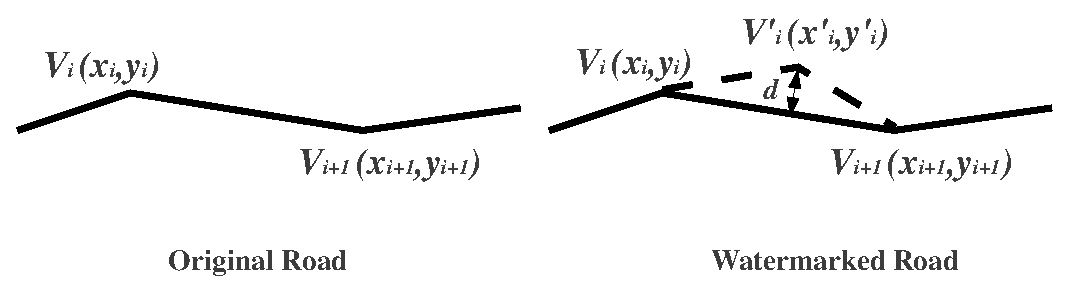
\epsfig{file=noise.eps,width=\columnwidth}
%\caption{Adding Vertex to Digital Road Map}
%\label{fig:11}
%\end{figure}
%Thus we can define the utility of the whole watermarked or attacked map as follows:
%
%\begin{eqnarray*}
%\Delta{R}_{i}'<\Delta{t}_{max}\\
%\frac {1}{N'}{\sum _{i=1}^{N'}{\Delta{R}_{i}'}}<\Delta{T}_{max}
%\end{eqnarray*}
%
%where $\Delta{t}_{max}$ gives the error bound for an individual road and $\Delta{T}_{max}$ gives the gobal 
%error bound for watermarking the whole digital road map. Here $\sum{\Delta{t}_{max}}\ge \Delta{T}_{max}$
%should be guaranteed, which means the sum of changes tolerance for all individual roads
% will be greater than the overall change tolerance in the map.
%

\subsection{Insertion and Detection of Watermarks}
Generally, the purpose of watermarking is to encode small amount of
{\em inperceivable} information into the map, 
and the detection process attempts to 
decode the extra information out of a given map and returns true if it is 
successful or false otherwise. 
The encoding and decoding processes generally need 
some secret keys to enhance the robustness of the watermarks 
to various attacks. 
For a digital road map $M$, watermark $W$, and some secret key $K$, the 
interface of watermarking process can be represented by two functions 
$\I$ and  $\D$.
\begin{eqnarray*}
\I &:& (M,~W,~K) \rightarrow M' \\
\D &:& (M,~W,~K) \rightarrow \{T~|~F\} 
\end{eqnarray*}
\noindent
where $M'$ is the watermarked map, %(illustrated in \figref{fig:11})
$\delta(M, M') \le \eta$, and detection process returns a boolean value
of either {\em true} or {\em false}.

%\begin{figure}[htb]
%\centering
%\epsfig{file=digitalwatermark.eps,width=\columnwidth}
%\caption{Inserting Watermark On Digital Road Map}
%\label{fig:11}
%\end{figure}

%Detection means trying to find the watermark which is encoded into a map and deciding whether 
%the map is watermarked or not. Only if knowing the watermarking strategy and the secret keys, 
%detection cound be performed successfully. For a watermarked map $M'$ the interface of detection 
%process could be denoted as follows. 
%\[Yes/No = Detection(M',~W,~Secret~Keys)\]


\subsection{Attacks}
%According to the data utility constraint in last subsection, if attackers want to change
%all data items, they can just change them slightly in order to keep the utility of the whole
%map, which will not beat most watermarking approaches.
%Therefore, attackers can select a small subset of the whole
%dataset to change and hope they can make the watermarking fail. 
%Because some secret keys are used in watermarking, attackers 
%can not know where the watermark is inserted and would randomly 
%select a subset to attack. For a digital road map:
%\begin{equation}
%\left\{
%\begin{array}{lcl}
%M &=& \bigcup _{i=1}^{N}{ {R}_{i} },{\rm where} ~N\ge 1 \\
%{R}_{i} &=& [ V_{i_1},~ V_{i_2}, \ldots, V_{i_m} ]
%\end{array}
%\right.
%\end{equation}
There are many different attacks on digital road map. In this section
We focus on into three types: the first type is a common attack which introduces
random noises into an illegal copy of the map. The other two types are more
complex attacks which involves cropping a given map into smaller pieces and merging
pieces together from various sources.

\subsubsection*{Noise Attack}
An attacker disturbs the watermarks in a map by selecting a subset of the nodes in
the map and perturb the position of these nodes slightly. The subset could be small
compared to the whole map: 
%This portion of data can be very small compared to the original dataset. By 
%add noise to the subset, the attacker hopes to render the watermark ineffective.
\[noise(M)= \{noise(R) ~|~ R \in M_1\} \cup M_2 \]
where
\begin{eqnarray*} 
M_1 \cap M_2 &=& \emptyset\\
M_1 \cup M_2 &=& M\\
noise(R) &=& [perturb(V)~ |~ V \in R].
\end{eqnarray*}
where $[f(V)~|~ V \in R ]$ a list comprehension constructed
from another list $R$.
%After attacking, for each road ${R}_{i}$, the vertice of it may unchange or just vary
%slightly.

\subsubsection*{Crop Attack}
An attacker crop a geographical region from the watermarked map and use it 
as if it's a new map. The crop attack can defeat almost all global 
watermarking techniques because the global information can be destroyed 
by the cropping. %\KZ{What about local watermarking?} 
Even for many local watermarking techniques, the resistance against cropping
is limited if just a small piece of the map is cropped.
We define cropping attack as:
\[
Crop(M) = \{ subseg(R) ~|~ R \in M'\}
\]
where 
$M' \subseteq M$ and $subseq (R)$ returns a subsequence of road $R$.

%After crop attack, we can get a ``partial'' map which is a subset of the original one.
%Each road in the new ``partial'' map is a $subseg$ of the corresponding road in the original
%map, which means that the vertices of new road is part of the original one. Accroding to 
%some special characteristics of digital road maps,
%an atackers can cause watermark failure by using 
%only a small portion of a digital road map. 
%If attackers select small portion of data, which means $n\ll N$ we 
If $M'$ is a very small subset of $M$, we call the attack ``massive crop'' attack.
None of the existing watermarking approaches can handle massive crop attack.

\begin{figure}[th]
\centering
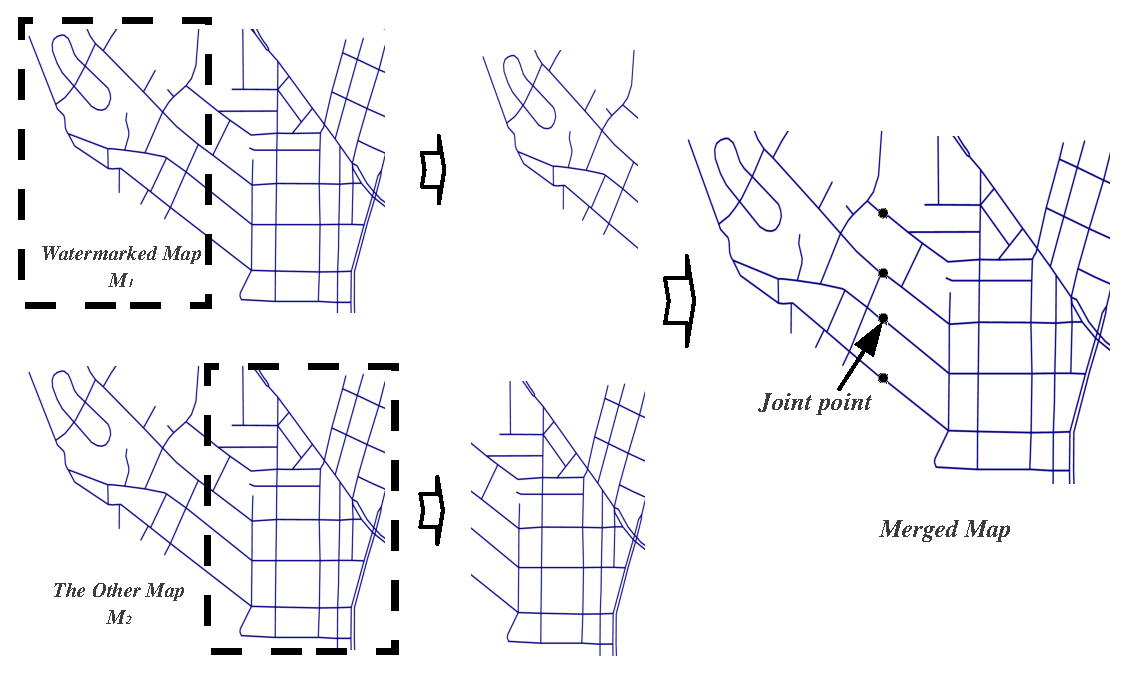
\epsfig{file=problem.eps, width=\columnwidth}
\caption{Merge Attack}
\label{fig:merge}
\end{figure}


\subsubsection*{Merge Attack}

This attack involves the merging of multiple maps from different sources
(see \figref{fig:merge}). Attackers can crop parts of different maps, and
joint those roads who is shared by these parts. 
%\KZ{Change this pic to something that can show
%how you merge the boundaries, and add a small paragraph to describe
%the common approach to merge two different maps.}
%Another special attack on digital road maps, which arises our 
%interests, will defeat most of these methods.
Maps from various sources differ by either precision of measurement, 
the granularity of road segmentation, 
or minor details of roads due to changes to the road
over time. However, maps of the same region will be largely identical.
This enables the attacker to crop parts from different maps and piece
them together to make a new map. There might some slight distortion or
inaccuracy at the boundaries but the resulting map is largely usable.
%Most of the digital road map vendors use paper road maps 
%as the basis for their digitized 
%road maps. The content of most paper maps is similar; the difference 
%is the map accuracy and the segmentation of long roads when a road map 
%is digitized. Digital road maps are actually only a little different digital 
%representation of same information. Thus, the digital road maps 
%from different vendors are similar for a specific area. Like figure 
%\ref{fig:12}, attackers can create their own digital road map 
%$W$ by partitioning different digital road maps and using one part from each map.
%Given a list of different maps ${M}_{i}$, $i\in[1,n]$, a ``new'' map $M'$ can be created
%by equation (\ref{merge}) as follows. For each submap cropped from different dataset.
%The intersection between them is either empty or a set consists of several vertices. 
%And each vertex is the unique one belong to a certain road. Here we assume that the index 
%is a unique attribute of a road, which means ${R}_{k}\in {M}_{i}$, and ${R}_{k}'\in{M}_{j}$ 
%represent the same road in the real world. This assumption will not make any disturb to the 
%defination of road map. 
We define the ``merge'' of two maps as:

\[
Merge(M_1, M_2) = M_{sep} \cup M_{con}
\]
where
\begin{eqnarray*}
M_{sep} &=& \{ R_1 ~|~ R_1 \in M_1~ {\rm and} \\
&& \hspace*{1cm} \forall R_2 \in M_2: connect(R_1, R_2) = false \} \\ 
&&\cup \\
&& \{ R_2 ~|~ R_2 \in M_2~ {\rm and}\\
&& \hspace*{1cm} \forall R_1 \in M_1: connect(R_1, R_2) = false \} \\
M_{con} &=& \{join(R_1, R_2) ~|~ \forall R_1 \in M_1, R_2 \in M_2, \\
&& \hspace*{1cm} connect(R_1, R_2) = true \} \\
\end{eqnarray*}
and $connect(R_1, R_2)$ is a boolean function that evaluates to true if
two roads have the same name and share an endpoint within certain tolerance
where $join(R_1, R_2)$ returns a road that joins two connected roads with the
same name. Note that road names are stores in the attribute data of the
maps. $M_{sep}$ and $M_{con}$ are two sets of roads that make up the merged map,
where $M_{sep}$ denotes those roads from the original maps which are disjoint
and $M_{con}$ denotes a set of roads from the boundaries of the two input maps
which are joined together. 
%{\rm where}~&&\\
%{ M }_{ i }'&=&Crop({ M }_{ i })\\
%{ M }_{ j }'&=&Crop({ M }_{ j })
%\end{eqnarray*}
%
%\begin{eqnarray*}
%{\rm where},~\forall k\in[1,N]&&\\
%\exists {V}_{k_x}&\in&{{ M }_{ i }'}\bigcap { M }_{ j }'\\
%{\rm if~and~only~if}&&
%\end{eqnarray*}
%
%\begin{equation}
%\left\{
%\begin{array}{lcl}
%{R}_{k}&\in& { M }_{ i }' \\
%{R}_{k}'&\in& { M }_{ j }'\\
%{V}_{k_x}&=&{R}_{k}\bigcap {R}_{k}'
%\end{array}
%\right.
%\end{equation}

The above attack remains an open problem because
1) all global watermarking schemes are susceptible to ``massive crop'' attack; 
2) most local watermarking methods have no knowledge which part of the
map has been attacked. 
%So even for most local watermarking algorithms, in this 
%situation, will fail to detect their watermark, since a suspicious map 
%consists of different parts from different maps, the watermark information 
%remained in the map would be very insignificant compared to the information 
%contained in the whole map.  As far as we know, there is still no watermarking 
%methods gives a solution to this problem.
%
%In recent years, some watermarking methods have been proposed
%in order to specify the copyright of digital vector maps\cite{DBLP:conf/vldb/AgrawalK02,DBLP:conf/soda/KhannaZ00,DBLP:conf/iwdw/SionAP02,DBLP:conf/sigmod/SionAP03}.Some methods insert watermarks into the maps with different geographical
%information, e.i. angles\cite{Kim10:Angles}, shapes\cite{Bird09:Shape}. However, to the best of our knowledge, 
%there is still no watermarking method that can survive ``massive rop'' attack and ``merge attack''successfully. 
In this paper, we focus our attention on the two most difficult attacks, 
``massive crop'' and ``merge attack'' defined above, 
and propose an effective approach to defeat these
attacks while also perform well against other traditional attacks.




%%% Local Variables:
%%% mode: latex
%%% TeX-master: "paper"
%%% End:
